\heada{MESH}{CANGle}
\hspace{1.0cm}{{ cang           \hfill}} \\{\smallskip}
\hspace{1.4cm}{{ node,(x(i),i=1,ndm),angle \hfill}} \\{\smallskip}
\hspace{1.4cm}{{ linear \hfill}} \\{\smallskip}
\hspace{1.8cm}{{ 1,x1,y1,angle1 \hfill}} \\{\smallskip}
\hspace{1.8cm}{{ 2,x2,y2,angle2 \hfill}} \\{\smallskip}
\hspace{1.4cm}{{ quadratic \hfill}} \\{\smallskip}
\hspace{1.8cm}{{ 1,x1,y1,angle1 \hfill}} \\{\smallskip}
\hspace{1.8cm}{{ 2,x2,y2,angle2 \hfill}} \\{\smallskip}
\hspace{1.8cm}{{ 3,x3,y3,angle3 \hfill}} \\{\smallskip}
\hspace{1.4cm}{{ surface \hfill}} \\{\smallskip}
\hspace{1.8cm}{{ 1,x1,y1,z1,angle1 \hfill}} \\{\smallskip}
\hspace{1.8cm}{{ 2,x2,y2,z2,angle2 \hfill}} \\{\smallskip}
\hspace{1.8cm}{{ 3,x3,y3,z3,angle3 \hfill}} \\{\smallskip}
\hspace{1.8cm}{{ 4,x4,y4,z4,angle4 \hfill}} \\{\smallskip}
\hspace{1.4cm}{{ cartesian \hfill}} \\{\smallskip}
\hspace{1.4cm}{{ pola,x0,y0 \hfill}} \\{\smallskip}
\hspace{1.4cm}{{ gap,value \hfill}} \\{\smallskip}
\hspace{1.4cm}{{ <etc.,terminate with a blank record> \hfill}}
\headb

The angle of a sloping boundary condition may be set
using the {\it cartesian} reference coordinates for a node.
The input values are saved in a file(s) and searched
\textit{after} the entire mesh is specified.
The data is order dependent with data
defined by {\tt ANGL}e processed first, {\tt EANG}le processed second and
the {\tt CANG}le data processed last.  The value defined last is used for
any analysis.
The data input by {\tt CANG} replaces previously assigned values.
Coordinate systems for the global and rotated axes are shown in Fig.
\ref{cang1}.

\begin{figure}[hb!]
\begin{center}
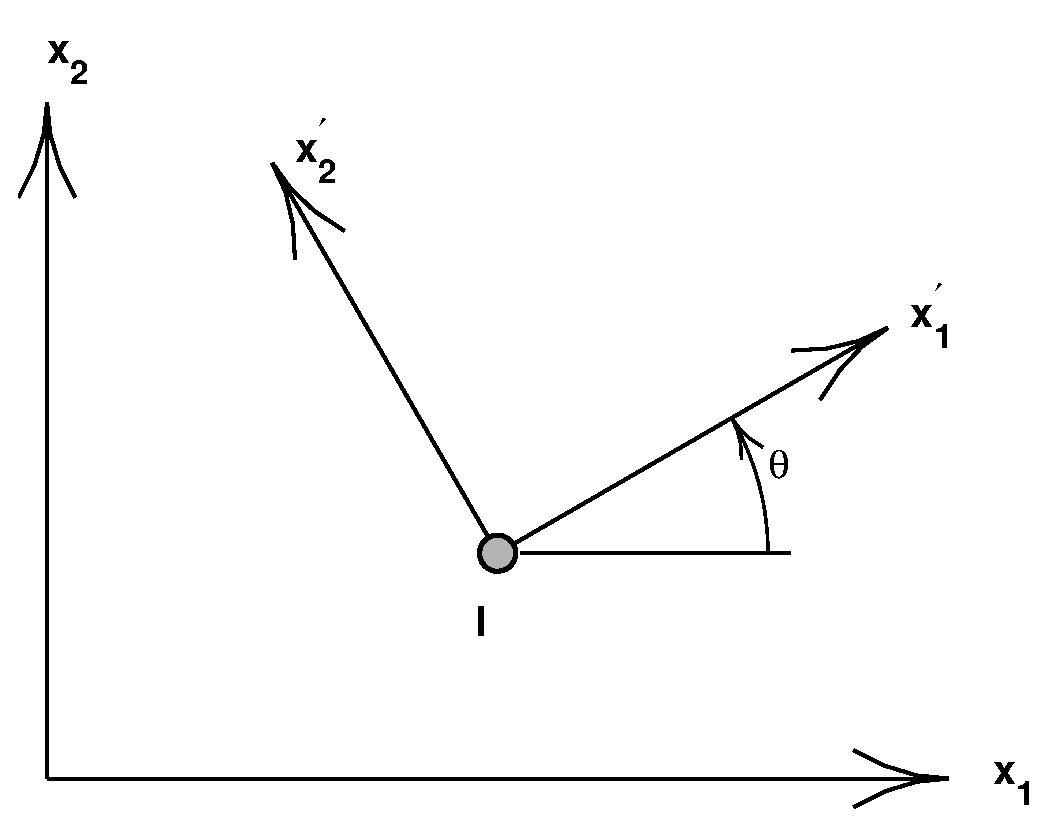
\includegraphics[width=3.5in]{../lmesh/angcor}
\caption{Coordinate rotation for node I.  \label{cang1} }
\end{center}
\end{figure}

For a single {\it node}, the data to be supplied during
the definition of the mesh consists of:

\begin{center}
\begin{tabular}{r l}
\it node   &-- Defines inputs to be for a {\it node} \\
\it x(1)   &-- Value of coordinates to be used during search \\
\it ...    &\quad (a tolerance of about 1/1000 of mesh size is \\
\it x(ndm) &\quad used during search, coordinate with smallest \\
           &\quad distance within tolerance is assumed to have \\
           &\quad specified value). \\
\it angle  &-- Value of the angle (in degrees) \\
\end{tabular}
\end{center}
At execution, the node(s) within the tolerance will have
their values set to the sloping condition.  For nodes with
sloping conditions, the degrees-of-freedom are expressed
with respect to the rotated frame instead of the global
frame.  For three dimensional problems the 3-direction
coincides with the x3-direction.

For two dimensional problems it is possible to
specify a segment to which the rotation angle is
applied.  The segment may be specified as a {\it linear}
or a {\it quadratic} line. For the {\it linear} segment the angle
is given together with the coordinates of the ends.
These are specified as:

\begin{verbatim}
       LINEar
         1,x1,y1,angle1
         2,x2,y2,angle1
\end{verbatim}

For {\it quadratic} segments the ends {\it (x1,y1)} and {\it (x2,y2)}
together with an intermediate point {\it (x3,y3)} are used.
The quadratic segment is given as:

\begin{verbatim}
       QUADratic
         1,x1,y1,angle1
         2,x2,y2,angle2
         3,x3,y3,angle3
\end{verbatim}

For three dimensional problems it is possible to
specify the segment to which the boundary conditions
are applied.  The segment is specified as a {\it surface}.
The data is specified as:

\begin{verbatim}
       SURFace
         1,x1,y1,z1,angle1
         2,x2,y2,z2,angle2
         3,x3,y3,z3,angle3
         4,x4,y4,z4,angle4
\end{verbatim}

The program assigns a search region and attempts to
find the elements and the nodes to which the specified
segments are associated.  It is possible that no segment
is located (an
error message will appear in the output file).  To
expand the search region a {\it gap} can be specified as:

\begin{verbatim}
       GAP,value}
\end{verbatim}
The {\it gap-value} is a coordinate distance within which
nodes are assumed to lie on the specified segment. The
value should be less than dimensions of typical elements
or erroneous nodes will be found by the search.
It is suggested that the computed boundary conditions
be checked graphically to ensure that they are
correctly identified (e.g., use {\tt PLOT,MESH} and {\tt PLOT,BOUN}dary
to show the locations of conditions).

The {\it polar} option may be used to set the origin {\it (x0,y0)} of a
polar coordinate system. Coordinates entered after
{\it polar} will be assumed to be radius and angle.  The
{\it cartesian} option resets the coordinate system to a
cartesian frame.

\noindent{\bf{Example: CANGle}}

In a two-dimesional problem
a rotated coordinate system of $45^o$ for a node located \textit{close} to the
coordinates $x_1 = 0$ and $x_2 = 5$ is desired.  The data may be specified
without needing to know a number for the node using the commands:
\begin{verbatim}
       CANGle
         NODE  0 5 45

\end{verbatim}
Note that the node \textit{closest} to this point will be selected. This can
be sensitive to roundoff if two nodes are at \textit{equal} distances from
the specified point.  Users should check (using graphics plot mode) that
the correct node(s) are selected.
\vfil\eject
